\documentclass[11pt]{article}

% ============================================================
%  Symbolic Regression of the cDFT--WSD surface-tension residual
%  for CO2-rich mixtures : V1 (physics-informed) vs V2 (composition)
% ============================================================

\usepackage[a4paper,margin=2.4cm]{geometry}
\usepackage{amsmath,amssymb}
\usepackage{booktabs}
\usepackage{array}
\usepackage{siunitx}
\usepackage{graphicx}
\usepackage{subcaption}
\usepackage[table]{xcolor}
\usepackage{caption}
\usepackage{microtype}
\usepackage[hidelinks]{hyperref}

\sisetup{
  round-mode          = figures,
  round-precision     = 4,
  table-number-alignment = center,
  exponent-product    = \cdot,
  detect-weight       = true
}

% --- notation shortcuts -------------------------------------
\newcommand{\eps}{\varepsilon}
\newcommand{\gcDFT}{\gamma_{\mathrm{cDFT}}}
\newcommand{\gbase}{\gamma_{\mathrm{base}}}
\newcommand{\xim}{x_{\mathrm{imp}}}
\newcommand{\yim}{y_{\mathrm{imp}}}
\newcommand{\zim}{z_{\mathrm{imp}}}
\newcommand{\dimp}{\Delta_{\mathrm{imp}}}
\newcommand{\lK}{\ell_K}
\newcommand{\Tr}{T_r}
\newcommand{\Prr}{P_r}
\newcommand{\omTr}{(1-T_r)}
\newcommand{\Pir}{\Pi}              % P / Psat0
\newcommand{\gr}{\gamma_r}
\newcommand{\drho}{\Delta\rho}
\newcommand{\drhon}{\Delta\rho^{\!*}}

\captionsetup{font=small,labelfont=bf}

\title{\textbf{Symbolic Regression of the cDFT--WSD Surface-Tension
Residual for CO\textsubscript{2}-Rich Mixtures}\\[4pt]
\large A Comparison of a Physics-Informed (V1) and a
Composition-Only (V2) Feature Set}
\author{Darshan Raju\\\small\texttt{rajudarshan1997@gmail.com}}
\date{June 3, 2026}

\begin{document}
\maketitle

\begin{abstract}
\noindent
We learn a closed-form correction to the uncorrected White-Bear / weighted
solvation-density (WSD) surface tension, so that it reproduces the full
classical density-functional-theory (cDFT) prediction for CO\textsubscript{2}-rich
mixtures. The learning target is the dimensionless \emph{relative residual}
$\eps=(\gcDFT-\gbase)/\gbase$. Two feature-engineering strategies are
compared under an identical train/validation/test protocol
($n=\num{23043}$, seed $5002034$): \textbf{V1}, a twelve-feature set that
augments the composition aggregates with physics-informed reduced state
variables (reduced temperature and pressure, saturation proximity, and the
Parachor density gap); and \textbf{V2}, a parsimonious five-feature
composition-only set. For each strategy we report the full Pareto frontier,
converting the symbolic-regression loss (mean squared error) to RMSE and
computing the per-complexity \emph{score} used for model selection.
Generalisation is assessed by 5-fold cross-validation using the same
stratified protocol as the GPR / SVGP residual surrogates. The selected
physics-informed V1 model is a compact rational form (complexity~12) with a
test $R^2=0.941$ on the residual and near-identical train/validation/test
scores; it reconstructs $\gcDFT$ to within $\SI{0.074}{mN\,m^{-1}}$ MAE.
Cross-validation of the V1 feature set gives $R^2=0.961\pm0.005$, confirming
its robustness. The interpretable V2 law, $\eps\approx-2.555\,\xim$, captures
the leading-order behaviour at complexity~4 with a test $R^2=0.618$.
\end{abstract}

% ============================================================
\section{Problem Statement and Target Definition}
% ============================================================

The baseline model is the uncorrected WSD surface tension,
$\gbase\equiv\gamma_{\mathrm{wsd}}^{\mathrm{UC}}$, and the reference is the
full cDFT prediction reconstructed as
\begin{equation}
  \gcDFT \;=\; \gamma_{\mathrm{wsd}}^{\mathrm{UC}}
  \;+\;\bigl(\gamma_{\mathrm{cDFT}}-\gamma_{\mathrm{wsd}}\bigr)_{\!\mathrm{uncorrected}} .
\end{equation}
Rather than regressing $\gcDFT$ directly, we regress the
\emph{dimensionless relative residual}
\begin{equation}
  \boxed{\;\eps \;=\; \frac{\gcDFT-\gbase}{\gbase}\;}
  \label{eq:target}
\end{equation}
so that the baseline carries the dominant signal and symbolic regression
need only describe the (small) physical correction. Predictions are mapped
back to dimensional surface tension through
\begin{equation}
  \widehat{\gcDFT} \;=\; \gbase\,\bigl(1+\widehat{\eps}\bigr),
  \label{eq:reconstruct}
\end{equation}
which makes the reported $\gcDFT$ metrics directly comparable to the
GPR/SVGP surrogates trained on the same data.

% ============================================================
\section{Data and Protocol}
% ============================================================

All cases are drawn from \texttt{CombinedDatasetSEC\_A4.csv}. After dropping
rows with missing or non-finite features the dataset contains
$n=\num{23043}$ points, split $70/15/15$ with a fixed
\texttt{MersenneTwister} seed of $5002034$:
\begin{center}
\begin{tabular}{lccc}
\toprule
 & Train & Validation & Test \\
\midrule
Rows & \num{16130} & \num{3456} & \num{3457} \\
\bottomrule
\end{tabular}
\end{center}
The split, seed, and target~\eqref{eq:target} are identical across both
feature sets, so any difference in performance is attributable solely to the
\emph{features} and the search budget.

% ============================================================
\section{Feature Engineering}
% ============================================================

The impurity is defined as every component other than CO\textsubscript{2}.
Liquid-, vapour-, and feed-phase impurity sums are formed as
$\xim=\sum_{i\neq\mathrm{CO_2}}x_i$,
$\yim=\sum_{i\neq\mathrm{CO_2}}y_i$, and
$\zim=\sum_{i\neq\mathrm{CO_2}}z_i$, together with the
phase-partitioning difference $\dimp=\xim-\yim$ and the impurity partition
coefficient $\lK=\ln\!\bigl[(\yim+\epsilon)/(\xim+\epsilon)\bigr]$ with
$\epsilon=10^{-12}$. These five \emph{composition aggregates} are common to
both versions.

\paragraph{V1 -- physics-informed (12 features).}
The composition aggregates are augmented with reduced state variables
referenced to pure CO\textsubscript{2}, motivated by the strong dependence of
surface-tension residuals on critical-point proximity and on the density gap
(Macleod--Sugden / Parachor variable):
\begin{align*}
  \Tr      &= T/T_{c}, &
  \omTr    &= 1-\Tr, &
  \Prr      &= P/P_{c}, \\
  \Pir     &= P/P_{\mathrm{sat}}^{0}, &
  \drho    &= \rho_l-\rho_v, &
  \drhon   &= \frac{\rho_l-\rho_v}{\rho_l^{0}-\rho_v^{0}}, \\
  \gr      &= \gamma_{\mathrm{wsd}}/\gamma^{0}_{\mathrm{CO_2}}. & & & &
\end{align*}

\paragraph{V2 -- composition-only (5 features).}
The five composition aggregates $\{\zim,\xim,\yim,\dimp,\lK\}$ only;
all state and density-gap variables are deliberately excluded to obtain a
maximally interpretable, composition-driven law.

Table~\ref{tab:notation} summarises the symbols used in the equations below.

\begin{table}[h]
\centering
\caption{Notation for the regressed features.}
\label{tab:notation}
\small
\begin{tabular}{ll@{\hskip 2.2em}ll}
\toprule
Symbol & Feature & Symbol & Feature \\
\midrule
$\xim$   & \texttt{x\_total\_impurity}     & $\Tr$    & \texttt{Tr} \\
$\yim$   & \texttt{y\_total\_impurity}     & $\omTr$  & \texttt{oneMinusTr} \\
$\zim$   & \texttt{z\_total\_impurity}     & $\Prr$    & \texttt{Pr} \\
$\dimp$   & \texttt{delta\_total\_impurity} & $\Pir$   & \texttt{P\_over\_Psat0} \\
$\lK$    & \texttt{logK\_total\_impurity}  & $\drho$  & \texttt{delta\_rho} \\
$\gr$    & \texttt{gamma\_base\_ratio}     & $\drhon$ & \texttt{delta\_rho\_norm} \\
\bottomrule
\end{tabular}
\end{table}

% ============================================================
\section{Symbolic Regression Configuration}
% ============================================================

Both runs use \texttt{SymbolicRegression.jl} with multithreaded
\texttt{equation\_search} over \num{200} iterations and protected operators.
The two configurations differ only in operator richness, population count
and the complexity ceiling (Table~\ref{tab:config}).

\begin{table}[h]
\centering
\caption{Search configuration for the two feature sets.}
\label{tab:config}
\small
\begin{tabular}{lcc}
\toprule
 & \textbf{V1} (physics-informed) & \textbf{V2} (composition) \\
\midrule
Binary operators & $+\,-\,\times$, \texttt{safepow}, \texttt{safe\_div}
                 & $+\,-\,\times$, \texttt{safepow}, \texttt{safe\_div} \\
Unary operators  & \texttt{abs}, \texttt{safe\_sqrt}, \texttt{safe\_log}
                 & \texttt{abs} \\
Populations      & 120 & 80 \\
Max.\ size       & 24  & 16 \\
Parsimony        & 0.003 & 0.003 \\
Batching         & 1000 & 1000 \\
\bottomrule
\end{tabular}
\end{table}

\subsection{Selection criterion: from loss to RMSE and score}

The search minimises the mean squared error of $\eps$, reported as the
\emph{loss} $L$. Because $L$ is a squared quantity we report the root mean
squared error
\begin{equation}
  \mathrm{RMSE} \;=\; \sqrt{L},
\end{equation}
which is on the same scale as $\eps$ itself. To rank Pareto-optimal
candidates we use the standard per-complexity \emph{score}, i.e.\ the rate at
which the loss decreases as one unit of complexity $c$ is added:
\begin{equation}
  \mathrm{score}_i \;=\;
  -\,\frac{\ln L_i-\ln L_{i-1}}{c_i-c_{i-1}} .
  \label{eq:score}
\end{equation}
A large score marks an equation whose added complexity is well justified by
the accuracy it buys; once the score collapses towards zero, further
complexity is essentially ``free-riding'' on overfitting. The final model is
chosen as the best trade-off between low RMSE and a still-meaningful score,
rather than the lowest-loss (largest) expression.

% ============================================================
\section{Pareto Frontiers}
% ============================================================

\subsection{V1 -- physics-informed}

Table~\ref{tab:paretoV1} lists the complete Pareto frontier. The score
\eqref{eq:score} is large at low complexity (a constant and the
$\ln(\drhon)$ family) and falls steeply beyond complexity~7. Around
complexity~10 the frontier transitions to a \emph{rational} form,
$\ln(\drhon)$ divided by a pressure/composition denominator, which carries
the accuracy-dominant tail. We select the \textbf{complexity-12} member
($\bigstar$): it is the simplest equation on this rational branch and sits at
the ``knee'' of the frontier, capturing $R^2=0.941$ with less than half the
complexity of the most accurate (complexity-24) expression, whose extra
terms buy only a further $\sim\!1.5$ points of $R^2$ (see
Sec.~\ref{sec:final}).

\begin{table}[h]
\centering
\caption{V1 Pareto frontier. $L$ is the SR loss (MSE of $\eps$);
RMSE and MAE are evaluated on the training set; score from
Eq.~\eqref{eq:score}. $\bigstar$ marks the selected equation.}
\label{tab:paretoV1}
\footnotesize
\renewcommand{\arraystretch}{1.18}
\begin{tabular}{c c c c c >{\raggedright\arraybackslash}p{7.2cm}}
\toprule
$c$ & RMSE & MAE & $L$ & score & Equation \\
\midrule
1  & 0.0849 & 0.0740 & \num{7.203e-3} & --   & $\drho$ \\
2  & 0.0431 & 0.0342 & \num{1.855e-3} & 1.357& $-0.0526$ \\
3  & 0.0239 & 0.0178 & \num{5.698e-4} & 1.180& $\ln(\drhon)$ \\
4  & 0.0170 & 0.0130 & \num{2.890e-4} & 0.679& $\drhon-1.0183$ \\
5  & 0.0141 & 0.0085 & \num{1.983e-4} & 0.377& $\ln(\drhon)-\xim$ \\
6  & 0.0127 & 0.0084 & \num{1.624e-4} & 0.199& $\drhon-(\xim+0.9979)$ \\
7  & 0.0124 & 0.0083 & \num{1.526e-4} & 0.062& $\bigl(\ln(\drhon)-\xim\bigr)\,\drhon$ \\
9  & 0.0123 & 0.0082 & \num{1.510e-4} & 0.005& $(\drhon-\drho)\,\ln(\drhon-\xim)$ \\
10 & 0.0111 & 0.0075 & \num{1.235e-4} & 0.202& $\ln(\drhon)\,/\,\sqrt{\Prr\,\gr}$ \\
\rowcolor{green!10}
12 & 0.0104 & 0.0071 & \num{1.082e-4} & 0.066& $\ln(\drhon)\,/\,\bigl[\sqrt{\Prr}+(\gr-\drhon)\bigr]$ \;$\bigstar$ \\
15 & 0.0097 & 0.0067 & \num{9.497e-5} & 0.044& $\Prr^{\,(1-\Tr)-\yim}\,\Tr\,\bigl(\ln(\drhon)-\xim\bigr)$ \\
16 & 0.0097 & 0.0066 & \num{9.410e-5} & 0.009& $\Prr^{\,-0.502\,\yim}\,\Tr\,\bigl(\ln(\drhon)-\xim\bigr)$ \\
17 & 0.0097 & 0.0065 & \num{9.356e-5} & 0.006& $\Tr\,\ln(\drhon-\xim)\,\sqrt{\Prr^{\,\dimp}-\zim}$ \\
18 & 0.0094 & 0.0065 & \num{8.893e-5} & 0.051& $\Prr^{\,(1.491-\gr)\dimp}\,\Tr\,\bigl(\ln(\drhon)-\xim\bigr)$ \\
19 & 0.0093 & 0.0061 & \num{8.569e-5} & 0.037& $\ln(\drhon)\,/\,\bigl[\Prr^{\,0.266}+\lK\bigl((\gr-\drhon)-\zim\bigr)\bigr]$ \\
21 & 0.0090 & 0.0060 & \num{8.047e-5} & 0.031& $\ln(\drhon)\,/\,\bigl[\Prr^{\,0.279}+\lK\bigl(\gr(\gr-\drhon)-\zim\bigr)\bigr]$ \\
23 & 0.0089 & 0.0059 & \num{7.878e-5} & 0.011& $\ln(\drhon)\,/\,\bigl[(\lK-\drhon)(\gr-\drhon)+\Prr^{\,0.352}-2\zim\bigr]$ \\
24 & 0.0088 & 0.0058 & \num{7.742e-5} & 0.017& $\ln(\drhon)\,/\,\bigl[\Prr^{\,0.279}+\lK\,\gr\bigl((\gr-\drhon)-\zim\bigr)\bigr]-0.0021$ \\
\bottomrule
\end{tabular}
\end{table}

\subsection{V2 -- composition-only}

The V2 frontier (Table~\ref{tab:paretoV2}) is dominated by a single sharp
score at complexity~2 and a strong secondary gain at complexity~4. Beyond
complexity~4 the RMSE plateaus near $0.027$: the additional terms reduce the
loss by less than \SI{15}{\percent} while quadrupling the complexity, so the
selected model is the complexity-4 linear law ($\bigstar$).

\begin{table}[h]
\centering
\caption{V2 Pareto frontier (columns as in Table~\ref{tab:paretoV1}).}
\label{tab:paretoV2}
\footnotesize
\renewcommand{\arraystretch}{1.18}
\begin{tabular}{c c c c c >{\raggedright\arraybackslash}p{7.2cm}}
\toprule
$c$ & RMSE & MAE & $L$ & score & Equation \\
\midrule
1  & 0.0909 & 0.0730 & \num{8.271e-3} & --    & $\xim$ \\
2  & 0.0431 & 0.0342 & \num{1.855e-3} & 1.495 & $-0.0526$ \\
\rowcolor{green!10}
4  & 0.0270 & 0.0180 & \num{7.291e-4} & 0.467 & $-2.5550\,\xim$ \;$\bigstar$ \\
5  & 0.0270 & 0.0180 & \num{7.291e-4} & 0.000 & $\xim/(-0.3914)$ \\
6  & 0.0270 & 0.0179 & \num{7.277e-4} & 0.002 & $\xim(\zim-2.5972)$ \\
7  & 0.0269 & 0.0178 & \num{7.222e-4} & 0.008 & $\xim/(-0.3492-\zim)$ \\
8  & 0.0268 & 0.0177 & \num{7.161e-4} & 0.008 & $\xim\bigl(-2.3588-\dimp^{2}\bigr)$ \\
9  & 0.0267 & 0.0177 & \num{7.151e-4} & 0.001 & $-2.3785\,\xim+0.0158\,\dimp$ \\
10 & 0.0265 & 0.0175 & \num{7.007e-4} & 0.020 & $-3.3478\,\yim^{\,\yim}\,\xim$ \\
11 & 0.0263 & 0.0174 & \num{6.925e-4} & 0.012 & $\bigl(-2.3320-|{-0.3671}-\dimp|\bigr)\xim$ \\
12 & 0.0262 & 0.0173 & \num{6.883e-4} & 0.006 & $(\yim-\zim)^{\yim}\,(-3.5244\,\xim)$ \\
13 & 0.0255 & 0.0168 & \num{6.505e-4} & 0.057 & $\xim\bigl(-1.7925-|\lK\dimp+1.0744|\bigr)$ \\
15 & 0.0254 & 0.0166 & \num{6.460e-4} & 0.003 & $\xim\bigl(-2.0208-|\yim+\dimp\lK+0.6315|\bigr)$ \\
16 & 0.0253 & 0.0166 & \num{6.417e-4} & 0.007 & $\xim\bigl(-1.9235-|{-0.5519}-\lK(\dimp+0.2337)|\bigr)$ \\
\bottomrule
\end{tabular}
\end{table}

% ============================================================
\section{Selected Models}
\label{sec:final}
% ============================================================

\paragraph{V1 (physics-informed), complexity 12.}
\begin{equation}
  \widehat{\eps}_{\mathrm{V1}}
  \;=\; \frac{\ln(\drhon)}
             {\sqrt{\Prr}\;+\;(\gr-\drhon)} .
  \label{eq:v1}
\end{equation}
The correction takes a compact \emph{rational} form: the numerator is the
logarithm of the normalised density gap $\drhon$ (Parachor variable), while
the denominator combines a square-root reduced-pressure term $\sqrt{\Prr}$
with the baseline-$\gamma$/density-gap difference $(\gr-\drhon)$. This links
the residual to interfacial density contrast (numerator) and to
pressure / density state (denominator) with only four variables and no fitted
constants. It is the simplest member of the rational branch of the frontier
and its train, validation and test scores agree to three decimals
($R^2 = 0.9416 / 0.9412 / 0.9408$), evidence that the form generalises rather
than memorises.

\paragraph{V2 (composition-only), complexity 4.}
\begin{equation}
  \widehat{\eps}_{\mathrm{V2}} \;=\; -2.5549\,\xim .
  \label{eq:v2}
\end{equation}
To leading order the residual is simply \emph{proportional to the
liquid-phase impurity fraction}: every percent of impurity in the liquid
lowers $\gcDFT$ relative to the WSD baseline by $\approx\SI{2.55}{\percent}$.

Table~\ref{tab:final} collects both selected equations side by side.

\begin{table}[h]
\centering
\caption{Selected equations for both versions.}
\label{tab:final}
\small
\renewcommand{\arraystretch}{1.4}
\begin{tabular}{c c c >{\raggedright\arraybackslash}p{7.6cm}}
\toprule
Version & $c$ & Test $R^2$ & Selected $\widehat{\eps}$ \\
\midrule
V1 & 12 & 0.941 &
  $\ln(\drhon)\,/\,\bigl[\sqrt{\Prr}+(\gr-\drhon)\bigr]$ \\
V2 & 4  & 0.618 & $-2.5550\,\xim$ \\
\bottomrule
\end{tabular}
\end{table}

% ============================================================
\section{Performance}
% ============================================================

Table~\ref{tab:perf} reports the held-out performance of the two selected
models, both in the dimensionless residual space ($\eps$) and after
reconstruction to surface tension via Eq.~\eqref{eq:reconstruct}.

\begin{table}[h]
\centering
\caption{Held-out performance of the selected V1 and V2 models.
Residual metrics are on $\eps$ (dimensionless); $\gcDFT$ metrics are in
\si{mN\,m^{-1}}.}
\label{tab:perf}
\small
\begin{tabular}{l S[round-precision=3] S[round-precision=3]
                  S[round-precision=4] S[round-precision=4]}
\toprule
& {V1 (test)} & {V2 (test)} & {V1 (val)} & {V2 (val)} \\
\midrule
$\eps$ $R^2$              & 0.9408 & 0.6181 & 0.9412 & 0.6207 \\
$\eps$ RMSE              & 0.01023 & 0.02599 & 0.01028 & 0.02612 \\
$\eps$ MAE              & 0.00698 & 0.01735 & 0.00711 & 0.01749 \\
$\gcDFT$ $R^2$           & 0.99943 & 0.99765 & 0.99945 & 0.99782 \\
$\gcDFT$ RMSE           & 0.1418 & 0.2891 & 0.1424 & 0.2824 \\
$\gcDFT$ MAE            & 0.0743 & 0.1618 & 0.0757 & 0.1606 \\
\midrule
Complexity              & {12} & {4}   & {12} & {4} \\
SR loss $L$             & \num{1.08e-4} & \num{7.29e-4} & & \\
\bottomrule
\end{tabular}
\end{table}

% ============================================================
\section{Cross-Validation}
% ============================================================

To assess generalisation independently of the single train/test split, each
feature set is evaluated by \textbf{5-fold cross-validation} using the same
protocol as the GPR / SVGP residual surrogates: a stratified $k$-fold over
T--P decile bins (shuffled, seed $4555525$). Because symbolic regression
refits the entire search each fold, the CV measures the generalisation of the
\emph{feature set and search} -- analogous to refitting the GPR kernel per
fold -- rather than of one fixed equation; within each fold the equation is
selected by an inner validation split (lowest validation RMSE). Scores are
reported as mean $\pm\,2\sigma$ across folds (Table~\ref{tab:cv}).

\begin{table}[h]
\centering
\caption{5-fold cross-validation (mean $\pm\,2\sigma$), $n=\num{23043}$,
200 iterations/fold. Residual metrics are on $\eps$; $\gcDFT$ metrics are in
\si{mN\,m^{-1}}. The last row is the per-fold selected complexity.}
\label{tab:cv}
\small
\renewcommand{\arraystretch}{1.25}
\begin{tabular}{l c c}
\toprule
 & \textbf{V1} (physics-informed) & \textbf{V2} (composition-only) \\
\midrule
$\eps$ $R^2$       & $0.961 \pm 0.005$       & $0.661 \pm 0.014$ \\
$\eps$ RMSE        & $0.00842 \pm 0.00058$   & $0.02494 \pm 0.00050$ \\
$\eps$ MAE         & $0.00568 \pm 0.00063$   & $0.01640 \pm 0.00051$ \\
$\gcDFT$ $R^2$     & $0.99965 \pm 0.00009$   & $0.99831 \pm 0.00030$ \\
$\gcDFT$ RMSE      & $0.113 \pm 0.015$       & $0.247 \pm 0.022$ \\
$\gcDFT$ MAE       & $0.0603 \pm 0.0061$     & $0.1434 \pm 0.0146$ \\
\midrule
Complexity / fold  & $22$--$24$              & $16$ \\
\bottomrule
\end{tabular}
\end{table}

The CV means track the single-split hold-out values in Table~\ref{tab:perf}
closely, and the $2\sigma$ bands are narrow, confirming that the V1-over-V2
advantage is not an artefact of the chosen split. The V2 CV $R^2$ ($0.661$)
exceeds its reported test value ($0.618$) only because the per-fold
auto-selection settles on complexity-16 expressions rather than the
hand-picked complexity-4 law of Eq.~\eqref{eq:v2}.

% ============================================================
\section{Diagnostic Plots of the Selected Equations}
% ============================================================

Figures~\ref{fig:parity} and~\ref{fig:residual} show the held-out behaviour
of the two \emph{selected} equations, Eqs.~\eqref{eq:v1} and~\eqref{eq:v2},
in the dimensionless residual ($\eps$) space. The parity plots
(Fig.~\ref{fig:parity}) overlay the train, validation and test splits against
the $y=x$ line with per-split $R^2$; the residual plots
(Fig.~\ref{fig:residual}) show the prediction error versus the predicted
value together with the $\pm\mathrm{RMSE}$ bands on the test and validation
splits.

\begin{figure}[h]
\centering
\begin{subfigure}[t]{0.49\textwidth}
  \centering
  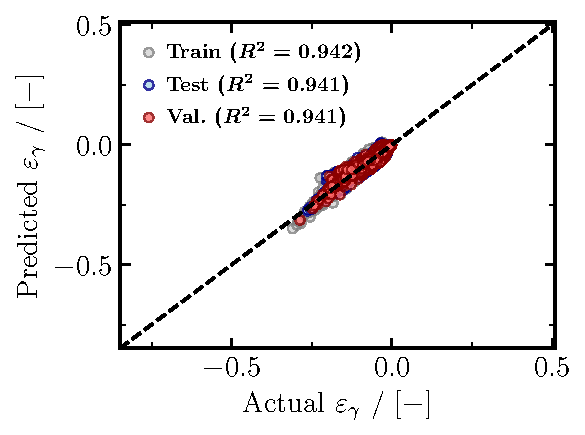
\includegraphics[width=\linewidth]{SR_MIXTURES_OUTPUTS/SR_parity_eps_base.pdf}
  \caption{V1 -- physics-informed (complexity 12).}
  \label{fig:parity-v1}
\end{subfigure}
\hfill
\begin{subfigure}[t]{0.49\textwidth}
  \centering
  
\includegraphics[width=\linewidth]{SR_MIXTURES_OUTPUTS_V2/SR_parity_eps_base.pdf}
  \caption{V2 -- composition-only (complexity 4).}
  \label{fig:parity-v2}
\end{subfigure}
\caption{Parity plots ($\widehat{\eps}$ vs $\eps$) of the selected equations.
The tighter clustering about $y=x$ for V1 reflects its higher test
$R^2=0.941$ relative to V2's $R^2=0.618$.}
\label{fig:parity}
\end{figure}

\begin{figure}[h]
\centering
\begin{subfigure}[t]{0.49\textwidth}
  \centering
  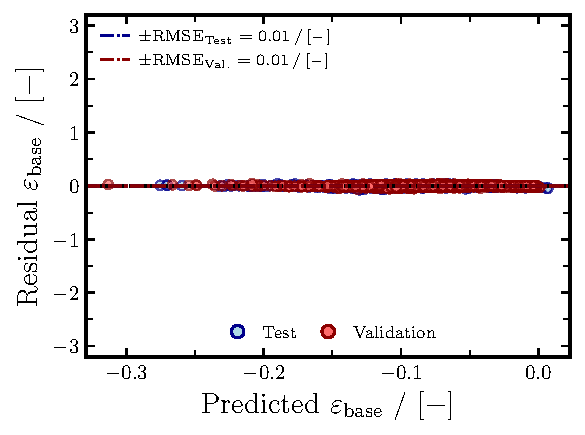
\includegraphics[width=\linewidth]{SR_MIXTURES_OUTPUTS/SR_residual_eps_base.pdf}
  \caption{V1 -- physics-informed (complexity 12).}
  \label{fig:residual-v1}
\end{subfigure}
\hfill
\begin{subfigure}[t]{0.49\textwidth}
  \centering
  
\includegraphics[width=\linewidth]{SR_MIXTURES_OUTPUTS_V2/SR_residual_eps_base.pdf}
  \caption{V2 -- composition-only (complexity 4).}
  \label{fig:residual-v2}
\end{subfigure}
\caption{Residual-vs-predicted plots of the selected equations, with the
$\pm\mathrm{RMSE}$ bands for the test and validation splits. The V1 band is
roughly three times narrower than V2's, consistent with the
$\eps$-RMSE values in Table~\ref{tab:perf}.}
\label{fig:residual}
\end{figure}

% ============================================================
\section{Discussion}
% ============================================================

\begin{itemize}
\item \textbf{Adding physics pays off in residual space.} Moving from the
composition-only V2 to the physics-informed V1 lifts the test $R^2$ on
$\eps$ from $0.618$ to $0.941$ and roughly halves the reconstructed
surface-tension error ($\SI{0.074}{mN\,m^{-1}}$ vs $\SI{0.162}{mN\,m^{-1}}$
MAE). The reduced state and density-gap variables therefore encode
information that pure composition cannot.

\item \textbf{Parsimony at the knee of the frontier.} The score
column~\eqref{eq:score} shows that the bulk of V1's accuracy is already
captured by complexity~$\le 7$, and the rational branch that begins near
complexity~10 adds a further jump. We deliberately select the
\emph{complexity-12} equation rather than the most accurate complexity-24
expression: the former reaches $R^2=0.941$ with a four-variable,
constant-free closed form, while doubling the complexity to~24 lifts $R^2$ to
only $0.956$ -- a $1.5$-point gain that does not justify the loss of
interpretability. Its train/validation/test scores agree to three decimals,
confirming the simpler form is not under-fitting in a fragile way.

\item \textbf{Cross-validation confirms the ranking is robust.} The 5-fold
CV (Table~\ref{tab:cv}) reproduces the hold-out gap with tight scatter:
the V1 feature set reaches $\eps$ $R^2=0.961\pm0.005$ versus V2's
$0.661\pm0.014$, and the small standard deviations show neither feature set
over-fits a particular split. The CV auto-selects the lowest-validation-RMSE
equation each fold (complexity~22--24 for V1, 16 for V2), so it measures the
generalisation of the \emph{feature set + search} and slightly exceeds the
parsimonious selected equations (V1 complexity~12, V2 complexity~4) reported
in Table~\ref{tab:final}.

\item \textbf{The honest comparison is in $\eps$ space.} In absolute
$\gcDFT$ both models exceed $R^2=0.997$, but this is largely inherited from
the WSD baseline through Eq.~\eqref{eq:reconstruct}. The residual-space
metrics expose the true gap between the two feature sets.

\item \textbf{V2 is the interpretable distillate.} Equation~\eqref{eq:v2}
gives a one-line physical statement -- the cDFT correction is, to first
order, linear in the liquid impurity fraction with slope $-2.55$ -- which is
valuable as a sanity check and a reduced-order model even though it is less
accurate.
\end{itemize}

% ============================================================
\section{Conclusion}
% ============================================================

Two symbolic-regression strategies were applied to the cDFT--WSD
surface-tension residual of CO\textsubscript{2}-rich mixtures under an
identical protocol. The physics-informed V1 model,
Eq.~\eqref{eq:v1}, a compact rational form, is the recommended predictive
correction (test $R^2=0.941$ on $\eps$, 5-fold-CV feature-set
$R^2=0.961\pm0.005$, $\SI{0.074}{mN\,m^{-1}}$ MAE on $\gcDFT$), chosen at the
knee of the Pareto frontier as the best balance of complexity, RMSE and
per-complexity score. The
composition-only V2 model, Eq.~\eqref{eq:v2}, is retained as a compact,
interpretable leading-order law. Together they bracket the
accuracy--interpretability trade-off of the surrogate correction.

\end{document}
